\section{Experiments}
\label{sec:experiments}

\subsection{Experimental Setup}
\label{sec:details}

% \textbf{Dataset Formation} 
% Approximately 3 million samples are used: Stage 1 comprises around 2.5 million, and Stage 2 has 1.3 million, with 800K overlapping. Data comes from a mix of open-source datasets like Midjourney~\citep{midjourney-niji-1m-llavanext} and CC12M~\citep{changpinyo2021cc12m}, and synthetic data created with publicly available T2I models, including Flux.1 dev~\citep{flux} and Stable Diffusion v3.5 Large~\citep{2024SD3}. More details are in \Cref{app:data_form} and \Cref{tab:dataset}.


\textbf{Implementation Details} 
The multimodal encoder is initialized using CLIP-Large-Patch14~\citep{Radford2021LearningTV} and Flant5-XL~\citep{flant5}, with a 224×224 image receptive field. 
The generator is initialized from LlamaGen-XL~\citep{llamagen}(775M). A two-layer MLP serves as the projector.
We freeze the encoder, training only the projector and generator for one epoch in Stage 1, then fine-tune the full model (except the vision encoder) for two more epochs in Stage 2.
Training on 8 A100 GPUs (80 GB each) takes about 1.5 days. More details are in \Cref{sec:Exp_Details}.
% To implement the MLP-based Projection, we train the MLP Projector on LLaVA-CC3M-Pretrain-595K data~\citep{liu2023llava}, keeping the vision and text encode frozen following the setting of LLAVA alignment training. For the Query-based Token Distillation, the model is initialized with BLIP2-Flant5-XL~\citep{li2023blip2}.

% \paragraph{Training Details}
% \label{sec:setup}


% To further investigate the effect of multi-image conditioning in multimodal generation, we continue training the model using a mixture of Stage 2 data and additional multi-subject samples generated via our data construction pipeline. In this setting, the model is tasked with reconstructing the original image based on segmented object crops and the corresponding image caption. Training is conducted for one additional epoch with a learning rate of 5e-5. Due to context length constraints, we limit each example to a maximum of three sub-images, resulting in a total sequence length of 888 tokens.

% \subsection{Evaluation Setup}


\textbf{Benchmark \& Metric.} We evaluate \model on \textbf{DreamBench}~\citep{ruiz2023dreamboothfinetuningtexttoimage} and \textbf{DreamBench\texttt{++}}~\citep{peng2025dreambenchpp} benchmarks.
\textbf{DreamBench} employs CLIP and DINO scores to measure the fidelity to images and prompts.
\textbf{DreamBench\texttt{++}} offers a scaled and diverse evaluation dataset and introduces a human-aligned automatic evaluation protocol using GPT-4o, addressing limitations of DreamBench evaluation.
GPT-4o evaluator scores generations on two axes: \textbf{Concept Preservation (CP)}, measuring the retention of the subject's visual identity, and \textbf{Prompt Following (PF)}, evaluating how accurately the image reflects the text prompt.
% Performance on DreamBench\texttt{++} is summarized by the combined CP$\cdotp$PF score, reflecting a balanced overall generation capability.
Details can be found in the \Cref{app:DreamBench_Plus}.

% \textbf{DreamBench} includes 30 subjects and 25 prompts, evaluating subject-driven generation via image–image and image–text similarity. It uses CLIP and DINO embeddings to compute subject fidelity (between the generated and reference image) and prompt fidelity (between the generated image and the prompt).

% \textbf{DreamBench\texttt{++}} significantly scales up the evaluation with 150 subjects and 1,350 prompts spanning photorealistic, stylistic, and imaginative settings. It uses GPT-4o as an automatic evaluator, scoring each image on two axes:

% \begin{itemize}
%     \item \textbf{Concept Preservation (CP):} Measures how well the generated image retains the visual identity of the reference subject (e.g., shape, color, texture, and facial details).
%     \item \textbf{Prompt Following (PF):} Evaluates how accurately the image reflects the semantics and context of the text prompt, including relevance, accuracy, and completeness.
% \end{itemize}


\textbf{Baselines.}
We compare our method against various baselines, categorized as follows:
\begin{itemize}[left=2pt, itemsep=0.5pt,topsep=0.5pt]
    \item \textbf{Fine-tuning-based methods:} Textual Inversion~\citep{gal2022imageworthwordpersonalizing}, and DreamBooth~\citep{peng2025dreambenchpp}, which fine-tune models with auxiliary control mechanisms on a subset of benchmark data.
    \item \textbf{Test Time Tuning-Free Methods:} Models pretrained on large-scale data and evaluated in a zero-shot. Diffusion-based models like BLIP-Diffusion~\citep{li2023blipdiffusionpretrainedsubjectrepresentation}, Emu2~\citep{emu2}, variants of IP-Adapter~\citep{ye2023ip-adapter}, and DreamEngine~\citep{dreamengine}, as well as autoregressive models like Unified-IO 2~\citep{lu2023unifiedio2} and Lumina-mGPT~\citep{2024lumina}. 
\end{itemize}

% \textbf{Baselines.} We compare our method against a range of baselines, categorized as follows:

% \noindent\makebox[2pt][l]{•}~\textbf{Fine-tuning-based methods.} Textual Inversion~\citep{gal2022imageworthwordpersonalizing} and DreamBooth~\citep{peng2025dreambenchpp}, which fine-tune models with auxiliary control mechanisms on subsets of benchmark data.

% \noindent\makebox[2pt][l]{•}~\textbf{Test-time tuning-free methods.} These models are pretrained on large-scale multimodal data and evaluated in a zero-shot setting without subject-specific fine-tuning. This category includes diffusion-based models such as BLIP-Diffusion~\citep{li2023blipdiffusionpretrainedsubjectrepresentation}, Emu2~\citep{emu2}, variants of IP-Adapter~\citep{ye2023ip-adapter}, and DreamEngine~\citep{dreamengine}, as well as autoregressive models like Unified-IO 2~\citep{lu2023unifiedio2} and Lumina-mGPT~\citep{2024lumina}.



\subsection{Main results}
\label{sec:main}
\Cref{tab:comparison} comprehensively evaluates our proposed autoregressive (AR) framework on the DreamBench++ benchmark, comparing it with diffusion-based and autoregressive-based baselines.
\model demonstrates highly competitive performance, particularly in achieving a strong balance between the guidance of both input modalities. Notably, this is achieved despite utilizing significantly fewer training resources and suboptimal model components compared to the state-of-the-art baselines.
% We assess performance along two key axes: Concept Preservation (CP)—measuring fidelity to the reference subject—and Prompt Following (PF)—evaluating semantic alignment with the textual prompt.

\textbf{Overall Performance.}
\model achieves a strong balance between concept fidelity and prompt alignment, resulting in the high \textbf{CP$\cdotp$PF} score. 
% Notably, even without task-specific fine-tuning and using a modest model size and training data, 
\model rivals fine-tuned methods like DreamBooth-LoRA, while significantly outperforming test-time tuning-free baselines such as Emu2 and DreamEngine. For instance, \model surpasses Emu2 in CP$\cdotp$PF score by approximately 30\%. 
% While fine-tuning methods like DreamBooth LoRA (0.52) achieve a higher CP$\cdotp$PF score, they benefit from training directly on the test set subjects, whereas our method operates in a test-time tuning-free manner.
A key strength of \model is its ability to harmoniously integrate multimodal inputs. Several strong baselines, including some AR methods like Lumina-mGPT and Unified-IO2, exhibit very high Concept Preservation (CP) but suffer from extremely low Prompt Following (PF), resulting in high \textbf{CP/PF} scores. This indicates a tendency to over-rely on the reference image while neglecting textual instructions. In contrast, \model delivers lowest CP/PF scores compared to all test-time tuning-free baselines, demonstrating effective and controlled integration of both visual and textual guidance.


\begin{table}[t]
\vspace{-8ex}
\centering
\small
\caption{
Comparison on DreamBench++. Models are ranked by \textbf{CP$\cdotp$PF}, indicating balanced overall multimodal image generation performance. \textbf{CP/PF} ratio reflects overfitting issue toward certain modality. ``*'' denotes model trained \textbf{from scratch}; others are adapted from pre-trained T2I models.
}

\label{tab:comparison}
\resizebox{\textwidth}{!}{%
\begin{tabular}{@{}l@{\hspace{1ex}}c@{\hspace{1ex}}c@{\hspace{1ex}}c@{\hspace{1ex}}c@{\hspace{1ex}}c@{\hspace{1ex}}c@{\hspace{1ex}}c@{\hspace{1ex}}c@{\hspace{1ex}}c@{\hspace{1ex}}c@{\hspace{1ex}}c@{\hspace{1ex}}c@{\hspace{1ex}}c@{\hspace{1ex}}c@{}}
\toprule
\textbf{Method} & \textbf{T2I Model} & \textbf{Train Data} & \textbf{Model Size} 
& \multicolumn{5}{c}{\textbf{Concept Preservation (CP)}} 
& \multicolumn{4}{c}{\textbf{Prompt Following (PF)}} 
& \textbf{CP$\cdotp$PF} & \textbf{CP/PF} \\
\cmidrule(lr){5-9} \cmidrule(lr){10-13}
& & & & \textbf{Animal} & \textbf{Human} & \textbf{Object} & \textbf{Style} & \textbf{Overall} 
& \textbf{Photo.} & \textbf{Style.} & \textbf{Imag.} & \textbf{Overall} & & \\
\midrule
\multicolumn{15}{c}{\textbf{Finetuned on Test Set}} \\
\midrule
Textual Inv.         & SD v1.5      & -     & 860M    & 0.50 & 0.36 & 0.31 & 0.36 & 0.38 & 0.67 & 0.69 & 0.44 & 0.62 & 0.24 & 0.61 \\
DreamBooth           & SD v1.5      & -     & 860M    & 0.64 & 0.20 & 0.49 & 0.48 & 0.49 & 0.79 & 0.78 & 0.50 & 0.72 & 0.36 & 0.68 \\
DreamBooth-L         & SDXL v1.0    & -     & 2.60B   & 0.75 & 0.31 & 0.54 & 0.72 & 0.60 & 0.90 & 0.90 & 0.75 & 0.87 & 0.52 & 0.69 \\

\midrule
\multicolumn{15}{c}{\textbf{Test-Time Tuning-Free Methods}} \\
\midrule
Unified-IO2*         & Unified-IO2  & 8.5B    & 7.00B   & 0.77 & 0.80 & 0.64 & 0.82 & 0.72 & 0.24 & 0.18 & 0.11 & 0.19 & 0.14 & 3.79 \\
Lumina-mGPT          & Chameleon    & 10M     & 7.00B   & 0.95 & 0.97 & 0.89 & 0.85 & 0.91 & 0.31 & 0.25 & 0.15 & 0.25 & 0.23 & 3.64 \\

DreamEngine          & SD3.5        & 21M     & 10.50B  & 0.76 & 0.72 & 0.61 & 0.73 & 0.68 & 0.44 & 0.37 & 0.25 & 0.37 & 0.26 & 1.84 \\

BLIP-Diffusion       & SD v1.5      & 130M    & 1.56B   & 0.67 & 0.56 & 0.47 & 0.51 & 0.55 & 0.58 & 0.51 & 0.30 & 0.50 & 0.27 & 1.10 \\

Kosmos-G             & SD v1.5      & 200M    & 3.00B   & 0.62 & 0.63 & 0.46 & 0.57 & 0.54 & 0.48 & 0.62 & 0.41 & 0.51 & 0.28 & 1.06 \\

IP-A-Plus ViT-H      & SDXL v1.0    & 10M     & 3.00B   & 0.90 & 0.85 & 0.76 & 0.91 & 0.83 & 0.50 & 0.38 & 0.28 & 0.41 & 0.34 & 2.02 \\

Emu2                 & SDXL v1.0    & 16M     & 37.00B  & 0.67 & 0.55 & 0.45 & 0.45 & 0.53 & 0.73 & 0.72 & 0.56 & 0.69 & 0.36 & 0.77 \\

IP-A ViT-G           & SDXL v1.0    & 10M     & 2.50B   & 0.67 & 0.56 & 0.50 & 0.75 & 0.59 & 0.74 & 0.63 & 0.45 & 0.64 & 0.38 & 0.92 \\
\rowcolor{gray!20} \model & LlamaGen & 3M      & 2.31B   & 0.65 & 0.36 & 0.57 & 0.47 & 0.55 & 0.86 & 0.85 & 0.80 & 0.84 & \textbf{0.47} & \textbf{0.65} \\
\bottomrule
\end{tabular}%
}
\end{table}



% Importantly, despite relying on a relatively low-quality image generator and sub-optimal encoders, our method excels in multimodal conditioning tasks. This suggests that the improved alignment and interaction between modalities enabled by our autoregressive design outweigh the limitations in token-level reconstruction quality inherent to discrete AR generation. As further shown in \Cref{tab:fid_comparison}, our model underperforms in traditional text-to-image metrics due to reconstruction loss and limited training data and model size; however, it excels in multimodal guidance, highlighting the core strength of our framework.
\textbf{Training Efficiency.}
A notable advantage of \model lies in its training efficiency. It is trained on only 3 million image-text pairs across two stages, substantially less than leading baselines, such as Emu2 (16M), Kosmos-G (200M), and DreamEngine (21M).
Beyond the reduced data requirements, the training process is highly resource-efficient: the entire training process completes in 1.5 days with 8 GPUs. This contrasts sharply with other baselines, such as Kosmos-G, which necessitates 256 GPUs over three days.
Despite this dramatically reduced computational and data budgets, \model achieves SOTA performance with balanced performance, highlighting its efficiency and effectiveness.
Furthermore, \model remains highly competitive in size compared to larger counterparts like Emu2 (37B parameters) and DreamEngine (10.5B parameters), highlighting our framework's effectiveness.


% These findings demonstrate that exposure to diverse object views during training improves the model’s ability to generalize visual identity under limited test conditions. Moreover, unlike many diffusion models that exhibit modality dominance (e.g., overemphasizing style or text), our AR framework integrates multiple inputs without sacrificing textual adherence—highlighting its scalability in complex multimodal scenarios.

% 

\textbf{Discussion and Connection to Methodology.}
The strong performance of \model — particularly its balanced multimodal generation and training efficiency — stems from its \textbf{autoregressive nature} and \textbf{two-stage training paradigm}.
The \textbf{autoregressive design}, which generates image tokens sequentially conditioned on a unified multimodal prefix, enables fine-grained, token-level alignment between inputs and outputs. This direct alignment significantly enhances prompt following, ensuring generated images accurately reflect both text and visual guidance.
The \textbf{two-stage training paradigm} is also critical for balanced multimodal control. It mitigates the common issue of over-reliance on one modality while ignoring others, resulting in significantly improved CP$\cdotp$PF scores compared to baselines.
Notably, \model achieves strong results despite using \textbf{relatively suboptimal components}.
While other baselines rely on advanced models such as Qwen-2.5 and SD3, we use Flan-T5 as the encoder and LlamaGen as the generator — both of which greatly underperform stronger counterparts, as shown in \Cref{tab:fid_comparison} and \Cref{tab:exp-geneval}. 
This highlights that our performance gains are driven by methodological strength, not from scaling up model capacity.
While performance on out-of-distribution or fine-grained categories remains limited due to the suboptimal components, \model maintains strong overall results by effectively integrate multimodal inputs for generation.




% The strong performance of our AR framework, especially its balanced CP and PF scores and high training efficiency, can be attributed to several key aspects of our methodology.
% The autoregressive nature of our method, which generates image tokens sequentially conditioned on a unified multimodal prefix, facilitates precise, token-level integration between the conditions and generated images. This direct alignment likely contributes to the high Prompt Following scores.
% Furthermore, our proposed two-stage training paradigm is crucial for achieving balanced multimodal control. 
% The first stage aims to enhances both pixel-level and semantic-level alignment, fostering better Concept Preservation. Stage 2 explicitly trains the model to effectively leverage and balance varied multimodal inputs
% It prevents the model from overemphasizing one modality (e.g., the reference image) at the expense of others (e.g., the text prompt), a common pitfall observed in other methods, and outperforms other baselines in CP$\cdotp$PF score.

% It is particularly noteworthy that our framework achieves impressive results despite using suboptimal components compared to others. For instance, we use a Flan-T5-XL as encoder, while others use more advanced models like Vicuna and Qwen-2.5. Additionally, our autoregressive generator (LlamaGen-XL) underperforms against advanced large scale diffusion models such as SDXL or SD3.5, and even earlier models like SD1.5. 
% This highlights the strength of our proposed framework. The direct multimodal alignment from the AR framework, and the significant impact of our two-stage training strategy in optimizing multimodal conditional image generation.

% Nevertheless, we acknowledge current limitations: due to the sub-optimal quality of our multimodal encoder and AR generator, performance on out-of-distribution or fine-grained human categories remains less robust. As shown in \Cref{tab:fid_comparison}, the text-to-image quality of our generation model lags behind SOTA diffusion models. However, the ability of our model to leverage multimodal inputs more effectively enables it to compensate for these weaknesses and maintain strong overall performance.

% Our results clearly demonstrate that the proposed autoregressive framework, even with modest data and compute resources, achieves state-of-the-art multimodal generation performance. Through architectural simplicity, efficient training, and balanced attention across modalities, our method offers a scalable and controllable alternative to diffusion-based approaches, setting a new standard for autoregressive multimodal image generation.








\subsection{Ablation Study}
\label{sec:ablation}

We conduct a ablation study on DreamBench++ and DreamBench focusing on two central questions: (1) How critical is Stage 1 for robust multimodal alignment? and (2) What role does each Stage 2 training task play in shaping model’s multimodal generation behavior?
Following prior work~\citep{peng2025dreambenchpp}, we report \textbf{CP$\cdot$PF} as a primary measure of multimodal image generation ability.
% We conduct the ablation study on both DreamBench++ and DreamBench benchmarks. Following prior work, we report the harmonic mean of Concept Preservation (CP) and Prompt Following (PF)—denoted as \textbf{CP$\cdotp$PF}—as a primary measure of multimodal generation quality. For all settings, we train for two epochs with consistent hyperparameters and average results over three random seeds. The results are presented in \Cref{tab:ablation_combined}.

\textbf{Importance of Stage 1: Foundational Multimodal Alignment.} \label{abl:stage1}
As shown in \Cref{tab:ablation_combined}, removing Stage 1 leads to the most severe performance drop, underscoring its foundational role. On DreamBench++, the CP score drops from 0.555 to 0.179, indicating a major loss in visual identity preservation, with PF also significantly reduced. Similar trends appear on DreamBench.
Ablating only \textbf{object segmentation task} in Stage 1 (\textit{w/o Obj. Seg. in Stage 1}) also hampers model performance.
While the remaining image reconstruction task supports pixel-level alignment, allowing for reconstruction of input images, it inadvertently leads the model to exhibit a copy-paste behavior, failing to capture semantic and visual information of input images. It confirms that reconstruction alone is insufficient for robust multimodal alignment.
Overall, these results highlight Stage 1 as critical for aligning multimodal inputs with output images.
Without such alignment, the model struggles to ground visual concepts from images, severely impairing its visual preservation ability.


\textbf{Contributions of Different Training tasks in Stage 2.} \label{abl:stage2} 
The distinct contributions of different Stage 2 tasks are also evident in \Cref{tab:ablation_combined}.
Excluding the \textit{Image Recovery} task leads to a sharp imbalance: while visual preservation metrics (CP, DINOv1, CLIP-I) show a notable increase, instruction following ability (PF and CLIP-T score) critically drops, showing an overfitting to visual features. This underscores that image recovery acts as a critical regularizer, encouraging the model to reconstruct incomplete visual contexts guided by text prompt, thereby fostering a balanced use of different modalities.
Conversely, ablating either the \textit{Object Segmentation} or the \textit{Subject-Driven Image generation} significantly degrades visual preservation ability, as these tasks prompt the model to utilize the visual features of the input image effectively to generate images.
Without these tasks, the model tends to over-rely on textual prompts, resulting in a regression towards a standard T2I model that neglects the reference image. 
These results highlight the importance of all Stage 2 tasks: image recovery ensures cross-modal balance, while object segmentation and subject-driven generation enhance the model’s ability to extract and utilize detailed visual information for image generation.
% It highlights the importance of object segmentation and subject-driven image generation in refining the model's ability to capture fine-grained visual details
% Although the instruction following ability seems slightly enhanced, it comes at the expense of neglecting visual features, resulting in generated images that often misaligned with the intended visual appearance from the input image. 
% Thus, object segmentation and subject-driven image generation are essential for enforcing spatial awareness and enhancing pixel-level subject integrity.

% \paragraph{Summary.}
% In essence, the ablation results confirm that all examined components of our two-stage training are vital. Stage 1 provides essential multimodal grounding, while each task in Stage 2 uniquely contributes to enhancing concept fidelity, ensuring textual adherence, or promoting a harmonious balance between them. Our model's superior performance is a direct outcome of this carefully orchestrated training strategy.



\begin{table}[t]
\vspace{-8ex}
\centering
\small
\caption{Ablation results on DreamBench++ and DreamBench.
% CP$\cdotp$PF denotes the harmonic mean between Concept Preservation (CP) and Prompt Following (PF). Our full model achieves the best trade-off across both benchmarks.
}
\label{tab:ablation_combined}
\resizebox{\linewidth}{!}{%
\begin{tabular}{lcccccc}
\toprule
\multirow{2}{*}{\textbf{Method}} &
\multicolumn{3}{c}{\textbf{DreamBench++}} &
\multicolumn{3}{c}{\textbf{DreamBench}} \\
\cmidrule(lr){2-4} \cmidrule(lr){5-7}
 & \textbf{CP} & \textbf{PF} & \textbf{CP$\cdotp$PF} 
 & \textbf{DINOv1} & \textbf{CLIP-I} & \textbf{CLIP-T} \\
\midrule
\textit{w/o Obj. Seg. in Stage 1}   
& $0.252 \pm 0.004$ & $0.479 \pm 0.005$ & $0.121$ 
& $56.113 \pm 0.082$  & $74.384 \pm 0.071$  & $23.965 \pm 0.038$ \\

\textit{w/o Stage 1 Alignment}     
& $0.179 \pm 0.002$ & $0.673 \pm 0.012$ & $0.120$ 
& $33.523 \pm 0.111$  & $67.705 \pm 0.101$  & $28.263 \pm 0.155$ \\

\textit{w/o Image Recovery}        
& $0.661 \pm 0.007$ & $0.284 \pm 0.004$ & $0.188$ 
& $74.471 \pm 0.321$ & $81.280 \pm 0.094$ & $24.210 \pm 0.022$ \\

\textit{w/o Object Segmentation}   
& $0.412 \pm 0.002$ & $0.918 \pm 0.003$ & $0.378$ 
& $57.221 \pm 0.119$  & $76.269 \pm 0.084$  & $31.078 \pm 0.050$ \\

\textit{w/o Multimodal T2I Task}   
& $0.407 \pm 0.004$ & $0.910 \pm 0.004$ & $0.370$ 
& $58.880 \pm 0.143$  & $76.529 \pm 0.102$  & $30.483 \pm 0.002$ \\

\rowcolor{gray!10}
\textbf{\model}         
& $0.555 \pm 0.006$ & $0.839 \pm 0.002$ & $\mathbf{0.466}$ 
& $70.853 \pm 0.327$  & $80.911 \pm 0.053$  & $29.071 \pm 0.080$ \\
\bottomrule
\end{tabular}%
}
\end{table}

\subsection{Analysis}
\label{sec:Analysis}

\textbf{Efficiency and Effectiveness: AR vs. Diffusion.}
To evaluate the efficiency of our AR framework against diffusion-based approaches, we conducted a controlled comparison with \textbf{Kosmos-G}~\citep{Kosmos-G}, a representative LMM-augmented diffusion model.Both models were trained from similar initializations on the same training data to ensure a fair comparison. Despite Kosmos-G employing a superior SD1.5 generator and Kosmos-1 as encoder, \model, which utilizes a underperformed LlamaGen generator and a FlanT5 based encoder, demonstrated significantly better performance on DreamBench++ as shown in \Cref{tab:comparison}.
It highlights the effectiveness of \model in fostering efficient multimodal learning and strong multimodal conditional generation.




\textbf{Comparison of Proposed Architecture Variants. }
As shown in \Cref{tab:ablation_combined}, we compare two architectural variants of \model: the MLP-based connector (\model) and a Query-based connector for the multimodal encoder. It reveals that an MLP-based connector significantly outperforms the query-based variant in CP scores, especially for humans and objects. It suggests that after visual token compression, the query-based approach struggles to retain fine-grained visual details, which are crucial for generative fidelity, even when guided by textual queries.
Nevertheless, due to effective token distillation, the Query-based variant facilitates training with multiple contextual images with minimal computational resources.
Despite these differences, both variants exhibit competitive performance compared to other baselines in \Cref{tab:comparison}. This demonstrates that our simple and coherent architecture can effectively propagate visual features, whether or not perform aggressive visual token compression, highlighting the flexibility and robustness of our framework.




% The MLP-based variant demonstrates superior performance, particularly in Concept Preservation. The Query-based variant suffers from a significant drop in CP, particularly for humans and objects. It suggests that after visual token compression, even when guided by textual queries, the model still loses fine-grained visual details crucial for generation fidelity.
% However, the Query-based variant, through token distillation, efficiently supports multi-image generation, enabling the training of a dozen of images for generation with the same computational resources. 
% \Cref{} illustrates examples of this multi-image generation using the Query-based variant.
% The MLP-based variant, designed to minimize information loss, effectively preserves visual details of reference images within our AR generation process.
% Despite these differences, both variants perform competitively compared to other baselines in \Cref{tab:comparison}. This confirms that our simple and coherent architecture allows for effective propagation of visual features throughout the generation process, with or without aggressive compression, enabling robust adaptation to various input formats.


% \begin{figure*}[tbhp]
% \centering
% \begin{minipage}[c]{0.42\textwidth}  % 改为 [c],垂直居中对齐
%     \centering
%     \captionof{table}{Image reconstruction performance (L2 distance) on COCO and JourneyDB datasets.}
%     \label{tab:reconstruct_l2}
%     \vspace{1ex}  % 可调整,增加表格与标题间距
%     \resizebox{\textwidth}{!}{
%     \begin{tabular}{@{}lcc@{}}
%     \toprule
%     \textbf{Method} & \textbf{COCO ($\downarrow$)} & \textbf{JourneyDB ($\downarrow$)} \\
%     \midrule
%     SeedTokenizer   & 0.5102 & 0.5291 \\
%     SEED-X          & 0.4317 & 0.4352 \\
%     EMU2-Gen        & 0.3828 & 0.2869 \\
%     DreamEngine     & \underline{0.2065} & \underline{0.2052} \\
%     \midrule
%     \textbf{Ours}   & \textbf{0.1008} & \textbf{0.0867} \\
%     \bottomrule
%     \end{tabular}
%     }
% \end{minipage}%
% \hfill
% \begin{minipage}[c]{0.56\textwidth}  % 同样改为 [c]
%     \centering
%     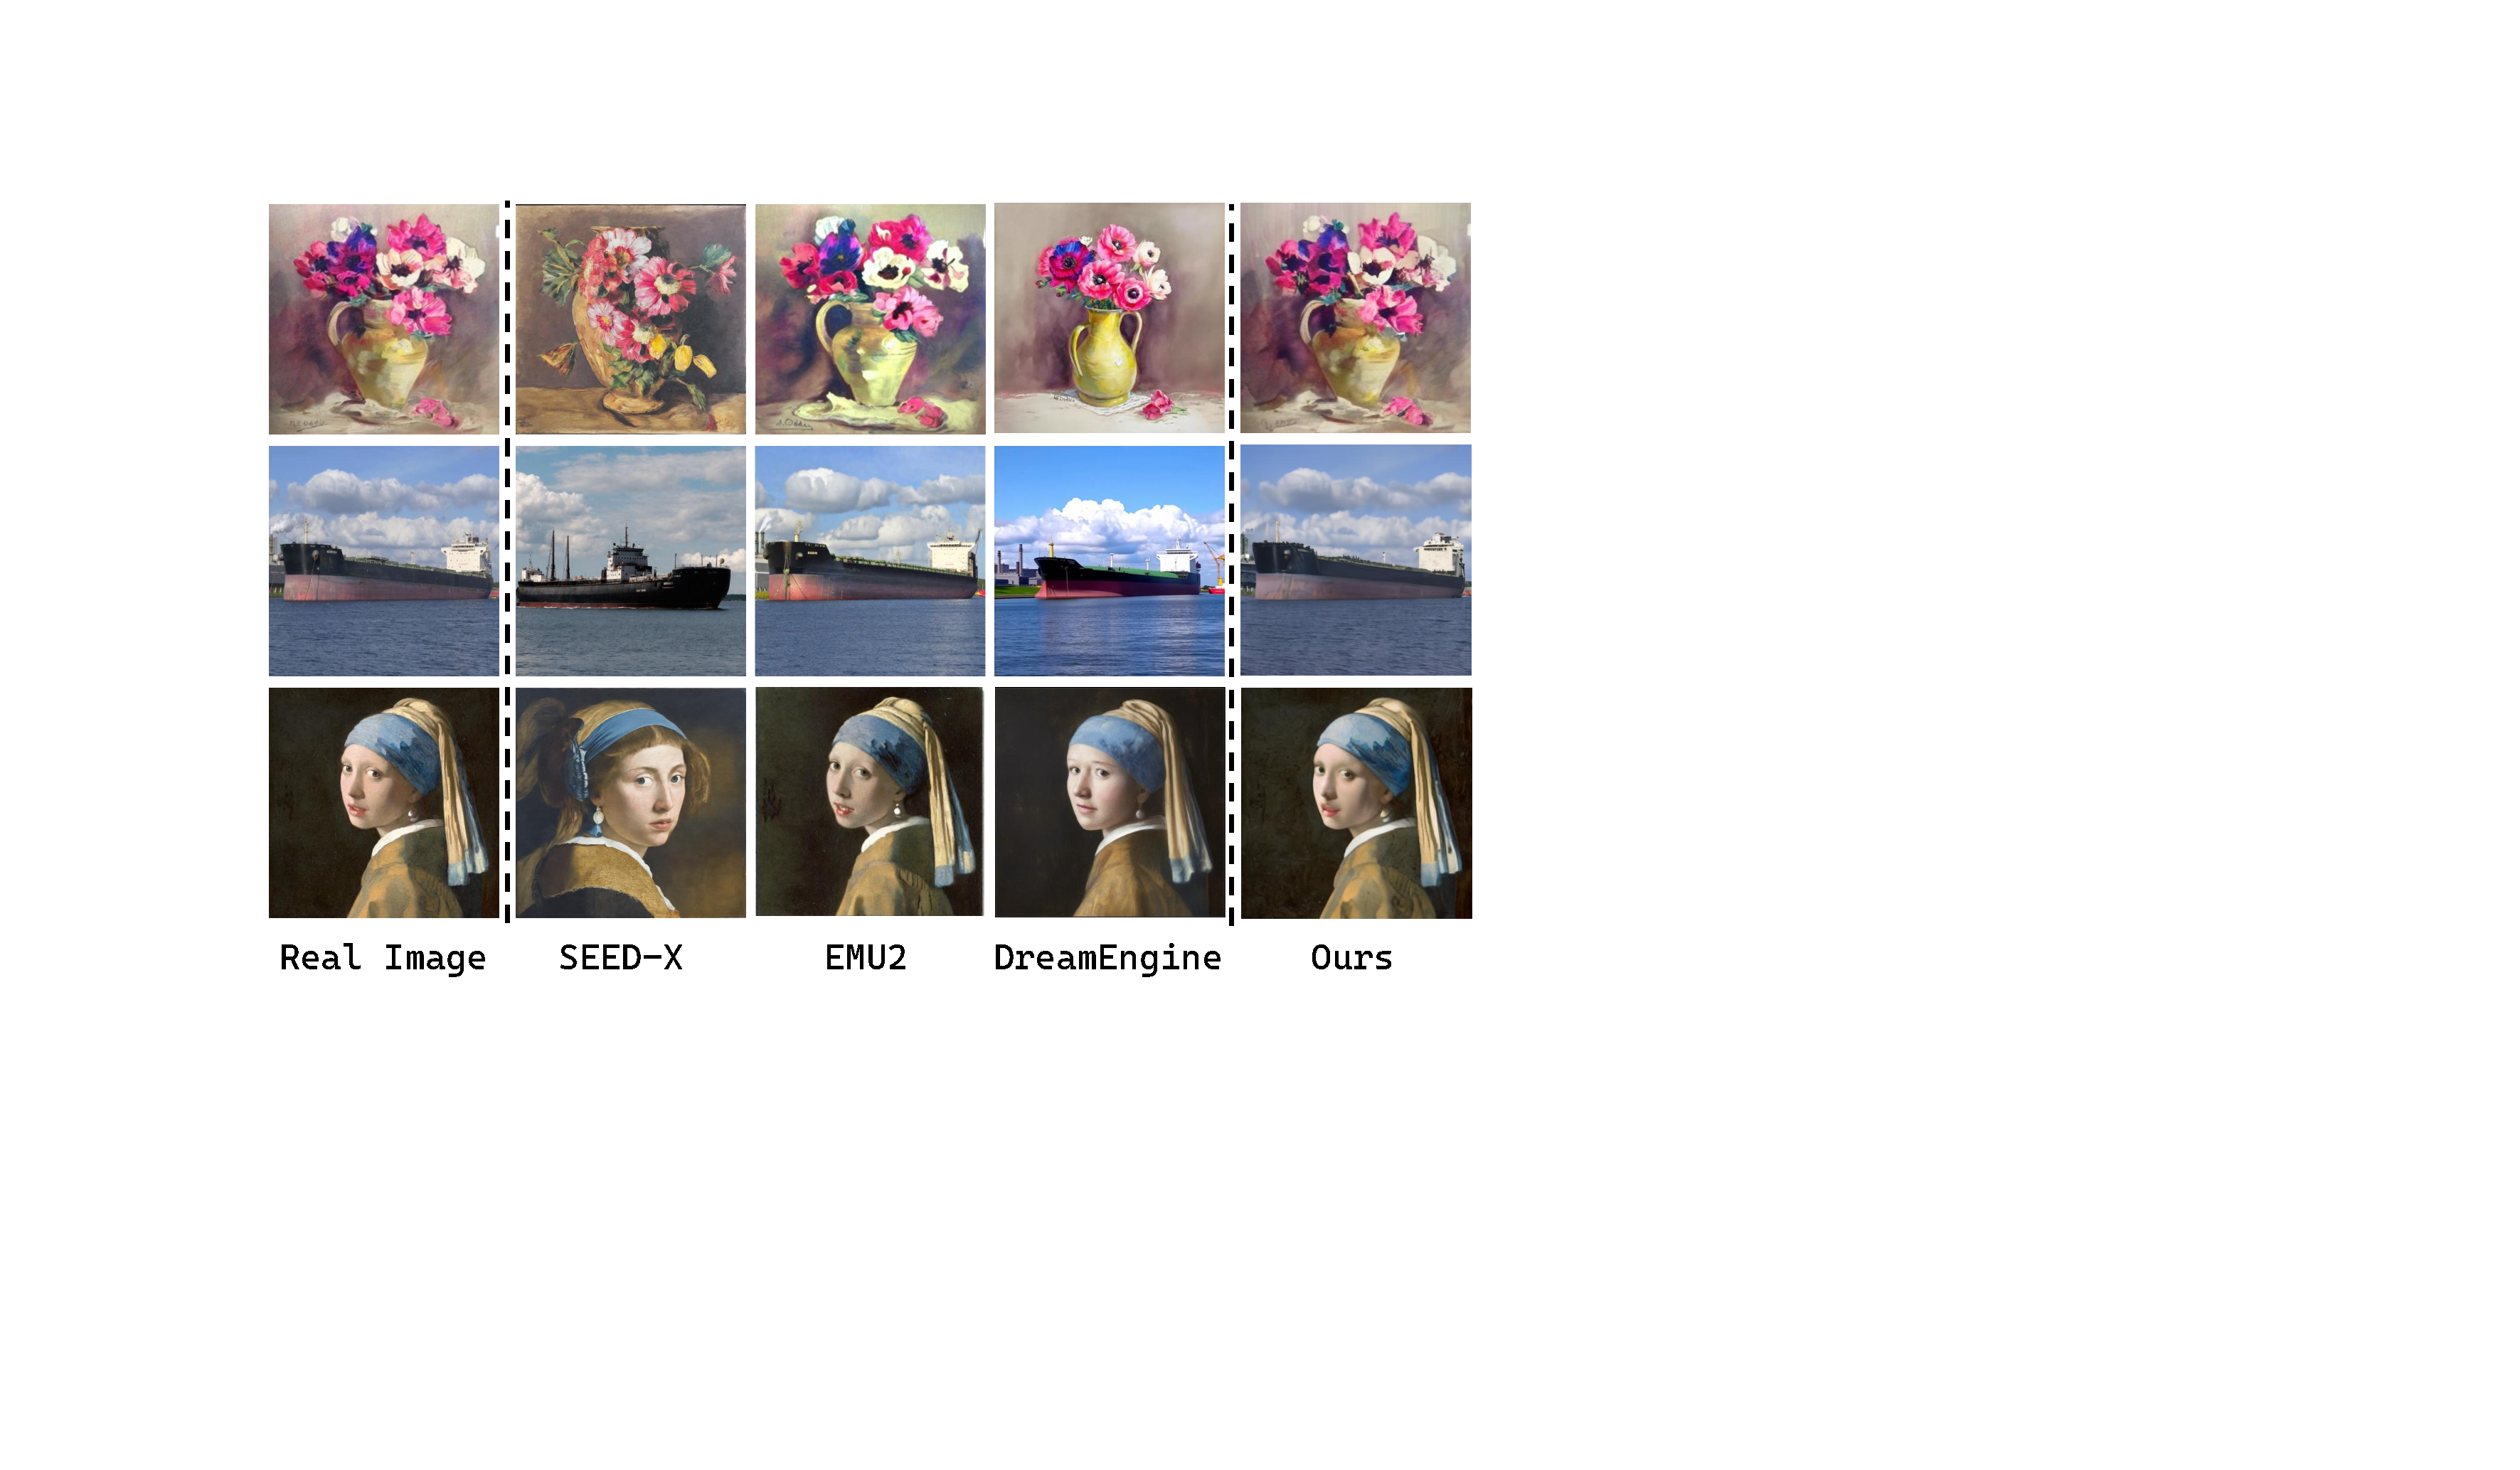
\includegraphics[width=\textwidth]{figures/reconstruction_exp.pdf}
%     \captionof{figure}{Image reconstruction results of various methods~\citep{dreamengine,2024SeedX,emu2}.}
%     \label{fig:reconstruction}
% \end{minipage}
% \end{figure*}



\begin{table}[t]
\vspace{-8ex}
\centering
\caption{Controllable experiments between \model and Kosmos-G in DreamBench++ benchmark.}
\label{tab:comparison}
\resizebox{\textwidth}{!}{%
\begin{tabular}{@{}lcccccccccc@{}}
\toprule
\textbf{Method} & \multicolumn{5}{c}{\textbf{Concept Preservation (CP)}} & \multicolumn{4}{c}{\textbf{Prompt Following (PF)}} & \textbf{CP$\cdotp$PF} \\ 
\cmidrule(lr){2-6} \cmidrule(lr){7-10}
 & \textbf{Animal} & \textbf{Human} & \textbf{Object} & \textbf{Style} & \textbf{Overall} & \textbf{Photorealistic} & \textbf{Style Transfer} & \textbf{Imaginative} & \textbf{Overall} & \\ 
\midrule
Kosmos-G  & 0.17 & 0.08 & 0.14 & 0.18 & 0.15 & 0.72 & 0.71 & 0.68 & 0.71 & 0.11 \\
\model     & 0.65 & 0.36 & 0.57 & 0.47 & \textbf{0.55} & 0.86 & 0.85 & 0.80 &\textbf{0.84} & \textbf{0.47} \\ 
\bottomrule
\end{tabular}%
}
\vspace{-2ex}
\end{table}


\begin{table}[t]
\centering
\vspace{-2ex}
\small
\caption{Ablation studies on architecture design and multi-image training}
\label{tab:ablation_combined}
\resizebox{\linewidth}{!}{%
\begin{tabular}{lcccccc}
\toprule
\multirow{2}{*}{\textbf{Method}} &
\multicolumn{3}{c}{\textbf{DreamBench++}} &
\multicolumn{3}{c}{\textbf{DreamBench}} \\
\cmidrule(lr){2-4} \cmidrule(lr){5-7}
 & \textbf{CP} & \textbf{PF} & \textbf{CP$\cdotp$PF} 
 & \textbf{DINOv1} & \textbf{CLIP-I} & \textbf{CLIP-T} \\
\midrule

\rowcolor{gray!10}
\textbf{\model}   
& $0.555 \pm 0.006$ & $0.839 \pm 0.002$ & $0.466$ 
& $70.853 \pm 0.327$  & $80.911 \pm 0.053$  & $29.071 \pm 0.080$ \\

\textit{w. Query-Variants}        
& $0.421 \pm 0.002$ & $0.882 \pm 0.000$ & $0.371$ 
& $54.518 \pm 0.317$  & $76.306 \pm 0.114$  & $30.792 \pm 0.040$ \\


\textit{w. Multi-image}         
& $0.586 \pm 0.006$ & $0.829 \pm 0.005$ & $\mathbf{0.486}$ 
& $72.487 \pm 0.147$ & $81.857 \pm 0.152$ & $28.545 \pm 0.043$ \\
\bottomrule
\end{tabular}%
}
\vspace{-2ex}
\end{table}


\textbf{Effect of Multi-Image Training.}
To assess the benefits of richer visual context, we further trained the model using a mix of Stage 2 data and additional multi-subject task(reconstructing images based on segmented objects and image caption) generated via our data construction pipeline. As shown in \Cref{tab:ablation_combined}, \textit{w. MultiImage Training} achieves a higher CP$\cdotp$PF score (0.49), improving CP to 0.60 while maintaining a strong PF score.
This emphasizes the advantage of enhanced visual context in training, prompting the model to efficiently handle and integrate information from multiple visual inputs, thereby improving its ability to preserve visual details in complex multimodal scenarios.

% To further investigate the effect of multi-image conditioning in multimodal generation, we continue training the model using a mixture of Stage 2 data and additional multi-subject samples generated via our data construction pipeline. In this setting, the model is tasked with reconstructing the original image based on segmented object crops and the corresponding image caption. Training is conducted for one additional epoch with a learning rate of 5e-5. Due to context length constraints, we limit each example to a maximum of three sub-images, resulting in a total sequence length of 888 tokens.



% \begin{table}[t]
% \centering
% \small
% \caption{Comparison of proposed variants across the DreamBench++ benchmark.}
% \label{tab:comparison}
% \resizebox{\textwidth}{!}{%
% \begin{tabular}{@{}lcccccccccc@{}}
% \toprule
% \textbf{Method} 
% & \multicolumn{5}{c}{\textbf{Concept Preservation (CP)}} 
% & \multicolumn{4}{c}{\textbf{Prompt Following (PF)}} 
% & \textbf{CP$\cdotp$PF} \\
% \cmidrule(lr){2-6} \cmidrule(lr){7-10}
% & \textbf{Animal} & \textbf{Human} & \textbf{Object} & \textbf{Style} & \textbf{Overall} 
% & \textbf{Photorealistic} & \textbf{Style Transfer} & \textbf{Imaginative} & \textbf{Overall} 
% & \\
% \midrule
% \rowcolor{gray!10} \textbf{Ours-MLP-based}       & 0.65 & 0.36 & 0.57 & 0.47 & 0.55 & 0.86 & 0.85 & 0.80 & 0.84 & \textbf{0.47} \\
% \rowcolor{gray!10} \textbf{Ours-Query-based}     & 0.54 & 0.32 & 0.38 & 0.38 & 0.42 & 0.91 & 0.91 & 0.78 & 0.88 & 0.37 \\
% \rowcolor{gray!10} \textbf{Ours-MultiImage}      & 0.71 & 0.40 & 0.60 & 0.52 & 0.60 & 0.86 & 0.85 & 0.80 & 0.83 & 0.49 \\
% \bottomrule
% \end{tabular}%
% }
% \end{table}


\begin{wrapfigure}{r}{0.52\textwidth}  % r 表示靠右,宽度根据内容调整
    \centering
    \vspace{-3ex}
    \begin{minipage}{0.9\linewidth}
        \centering
        \footnotesize
        \captionof{table}{Image reconstruction performance.}
        \vspace{-1ex}
        \label{tab:reconstruct_l2}
        \resizebox{\linewidth}{!}{
        \begin{tabular}{@{}lcc@{}}
        \toprule
        \textbf{Method} & \textbf{COCO ($\downarrow$)} & \textbf{JourneyDB ($\downarrow$)} \\
        \midrule
        SeedTokenizer   & 0.5102 & 0.5291 \\
        SEED-X          & 0.4317 & 0.4352 \\
        EMU2-Gen        & 0.3828 & 0.2869 \\
        DreamEngine     & \underline{0.2065} & \underline{0.2052} \\
        \midrule
        \textbf{\model}   & \textbf{0.1008} & \textbf{0.0867} \\
        \bottomrule
        \end{tabular}
        }
    \end{minipage}
    \vspace{1ex}
    
    \begin{minipage}{\linewidth}
        \centering
        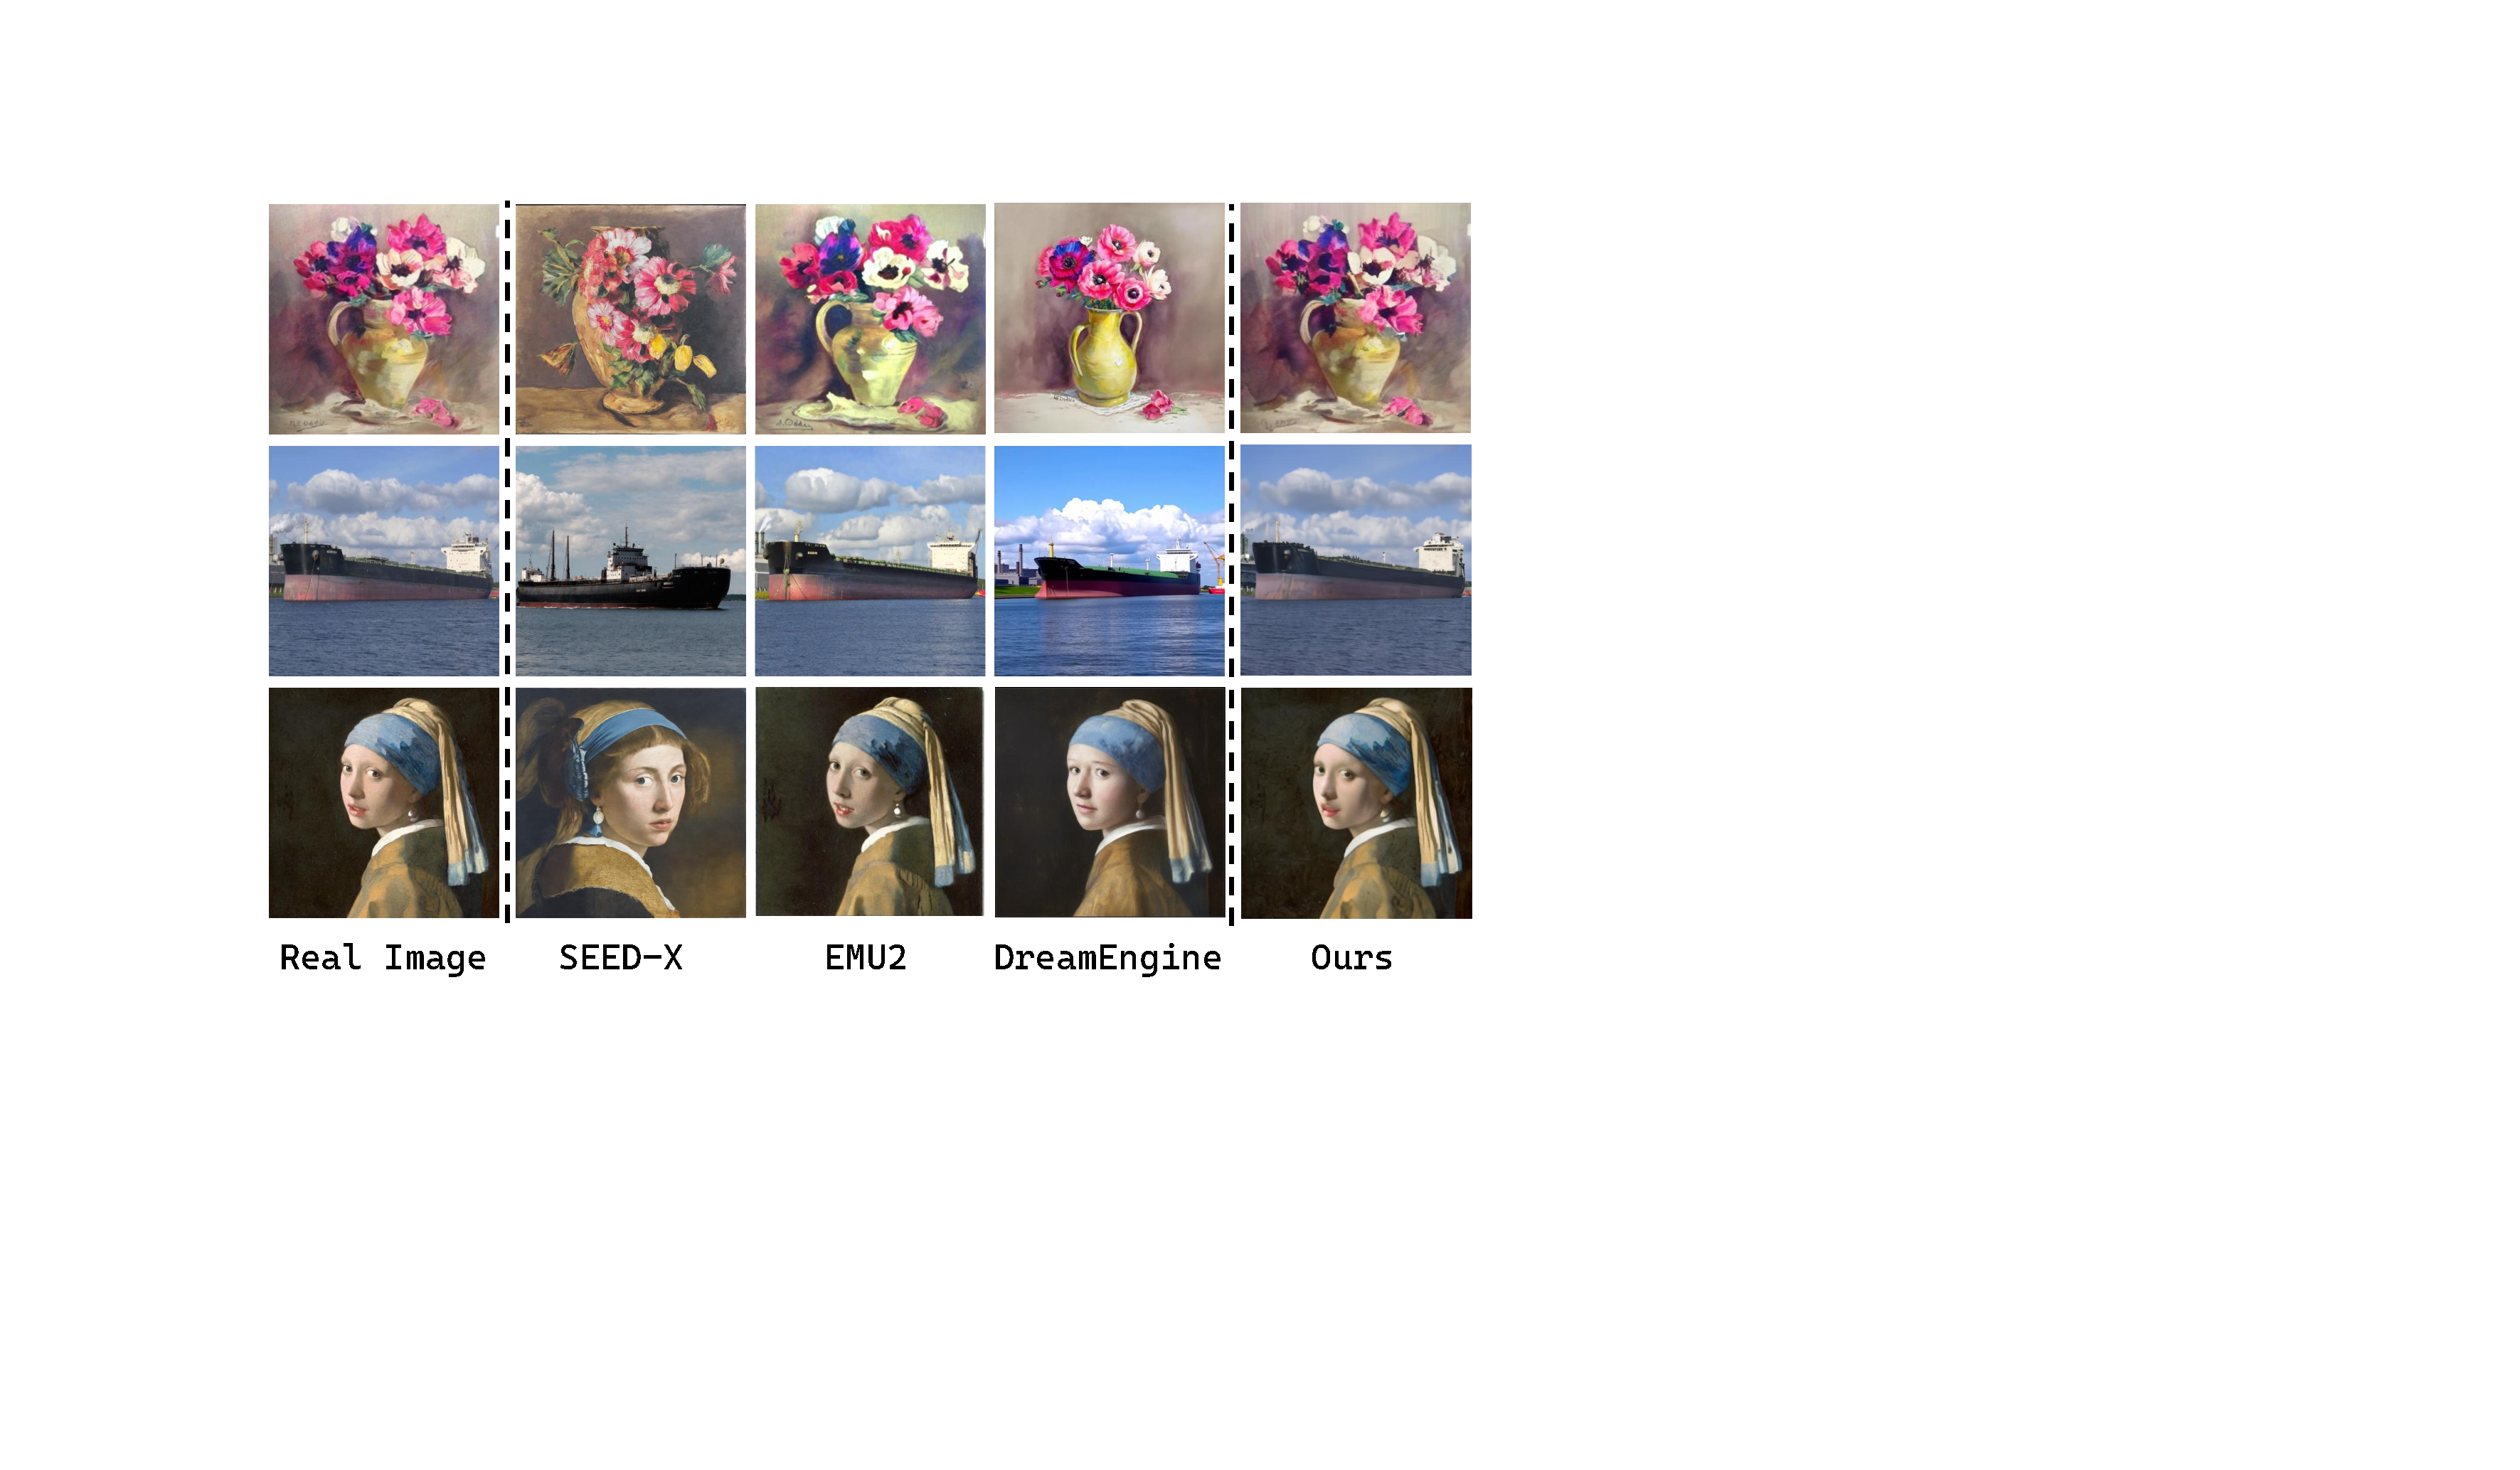
\includegraphics[width=\linewidth]{figures/reconstruction_exp.pdf}
        \vspace{-3ex}
        \captionof{figure}{Qualitative study on Image Reconstruction.}
        \label{fig:reconstruction}
    \end{minipage}
    \vspace{-5ex}

\end{wrapfigure}

\textbf{Image Reconstruction Fidelity.}
To quantify visual detail preservation in our framework, we evaluate \model on the Image Reconstruction Benchmark~\citep{dreamengine}, which measures similarity between input and reconstructed images. After fine‑tuning on reconstruction task for 1{,}000 steps, we compare the generated outputs with their originals using pixel‑space $\ell_2$ distance, following pervious work~\citep{dreamengine}. As shown in \Cref{tab:reconstruct_l2}, \model outperforms strong baselines with comparable architectures—SeedTokenizer~\citep{seed-tokenizer}, EMU2~\citep{emu2}, SeedX~\citep{2024SeedX}, and DreamEngine~\citep{dreamengine}—all of which couple LMMs with diffusion backbones.
\model achieves the best reconstruction quality, exceeding the second-best by 50\%, even with a $224{\times}224$ receptive field, while others varied from 384x384 to 512x512.
% In particular, it improves upon the second‑best approach by 51.2\% (COCO) and 57.7\%(JourneyDB) in $\ell_2$ distance, demonstrating superior pixel-level fidelity even with a $224{\times}224$ receptive field, while others range from 384x384 to 512x512. 
These gains confirm our model’s effectiveness at conditioning on—and faithfully reproducing—visual inputs.




% We introduce an  to evaluate the preservation of visual features in our Image-to-Image alignment task. This capability is essential for generating images conditioned on input images. 
% Afte finetuning on image reconstrction task for 1000 steps, we assess the similarity between the original and reconstructed images generatd by our model using the CLIP~\citep{radford2021clip} score and L2-Distance from the images in JourneyDB and COCO dataset. As shown in \Cref{tab:reconstruct}, we compare the performance of our model against several baselines with similar architectures, including SeedTokenizer~\citep{seed-tokenizer}, EMU-2~\citep{emu2}, SeedX~\citep{2024SeedX}, and DreamEngine~\citep{dreamengine}, which also integrate LMMs and diffusion models for generation. The results demonstrate that our model achieves the best average image reconstruction performance across both subsets of the benchmark. It notably surpasses the second-best by xx on the COCO and xx on the JourneyDB subsets in terms of L2 distance, highlighting its pixel-level consistency, albeit at an image receptive field of 224×224, while others varied from 384x384 to 512x512.


\textbf{Versatility Across Different Multimodal Tasks.}
To explore broader applicabilities of our framework, we evaluate its adaptability across diverse generation tasks, including image segmentation,  multi-image generation and multimodal in-context image generation. This was achieved with brief fine-tuning on relevant datasets, as detailed in~\Cref{app:applications}. Qualitative results in \Cref{fig:examples} show that the \model produces coherent, high-quality outputs that adhere to the provided constraints without requiring any architectural modifications. While achieving  performance in each specific domain would necessitate more specialized training and potentially more powerful multimodal encoder and generator components, these initial results underscore our framework's versatility and its potential as an effective foundation for a variety of multimodal conditional image generation applications.
 

% \paragraph{\mbox{Text-to-Image Generation}}

% We evaluate the text-to-image generation capability of our model on the COCO-40K benchmark. The results are presented in Table \ref{tab:fid_comparison}. Built upon the LlamaGen model~\citep{llamagen}, limited by the performance of the generator, our model shows much lower text-image generation ability than other baselines. However, thanks to the effective understanding of multimodal input, our model can balance these two different modalities, and with high-quality instruction following ability, ultimately further exceed other baselines in multimodal conditional image generation.
%  image segmentation set where? show cases additional task, editing; 



% \begin{table}[t]
% \centering
% \caption{Image reconstruction performance (L2 distance) on COCO and JourneyDB datasets.}
% \label{tab:reconstruct_l2}
% \resizebox{0.5\textwidth}{!}{
% \begin{tabular}{@{}lcc@{}}
% \toprule
% \textbf{Method} & \textbf{COCO ($\downarrow$)} & \textbf{JourneyDB ($\downarrow$)} \\
% \midrule
% SeedTokenizer              & 0.5102          & 0.5291          \\
% EMU2-Gen                  & 0.3828 & 0.2869 \\
% SEED-X                    & 0.4317          & 0.4352          \\
% DreamEngine               & \underline{0.2065}          & \underline{0.2052}          \\
% \midrule
% \textbf{Ours}             & \textbf{0.1008} & \textbf{0.0867} \\
% \bottomrule
% \end{tabular}
% }
% \end{table}



% \begin{figure*}[htbp]
% \centering
% 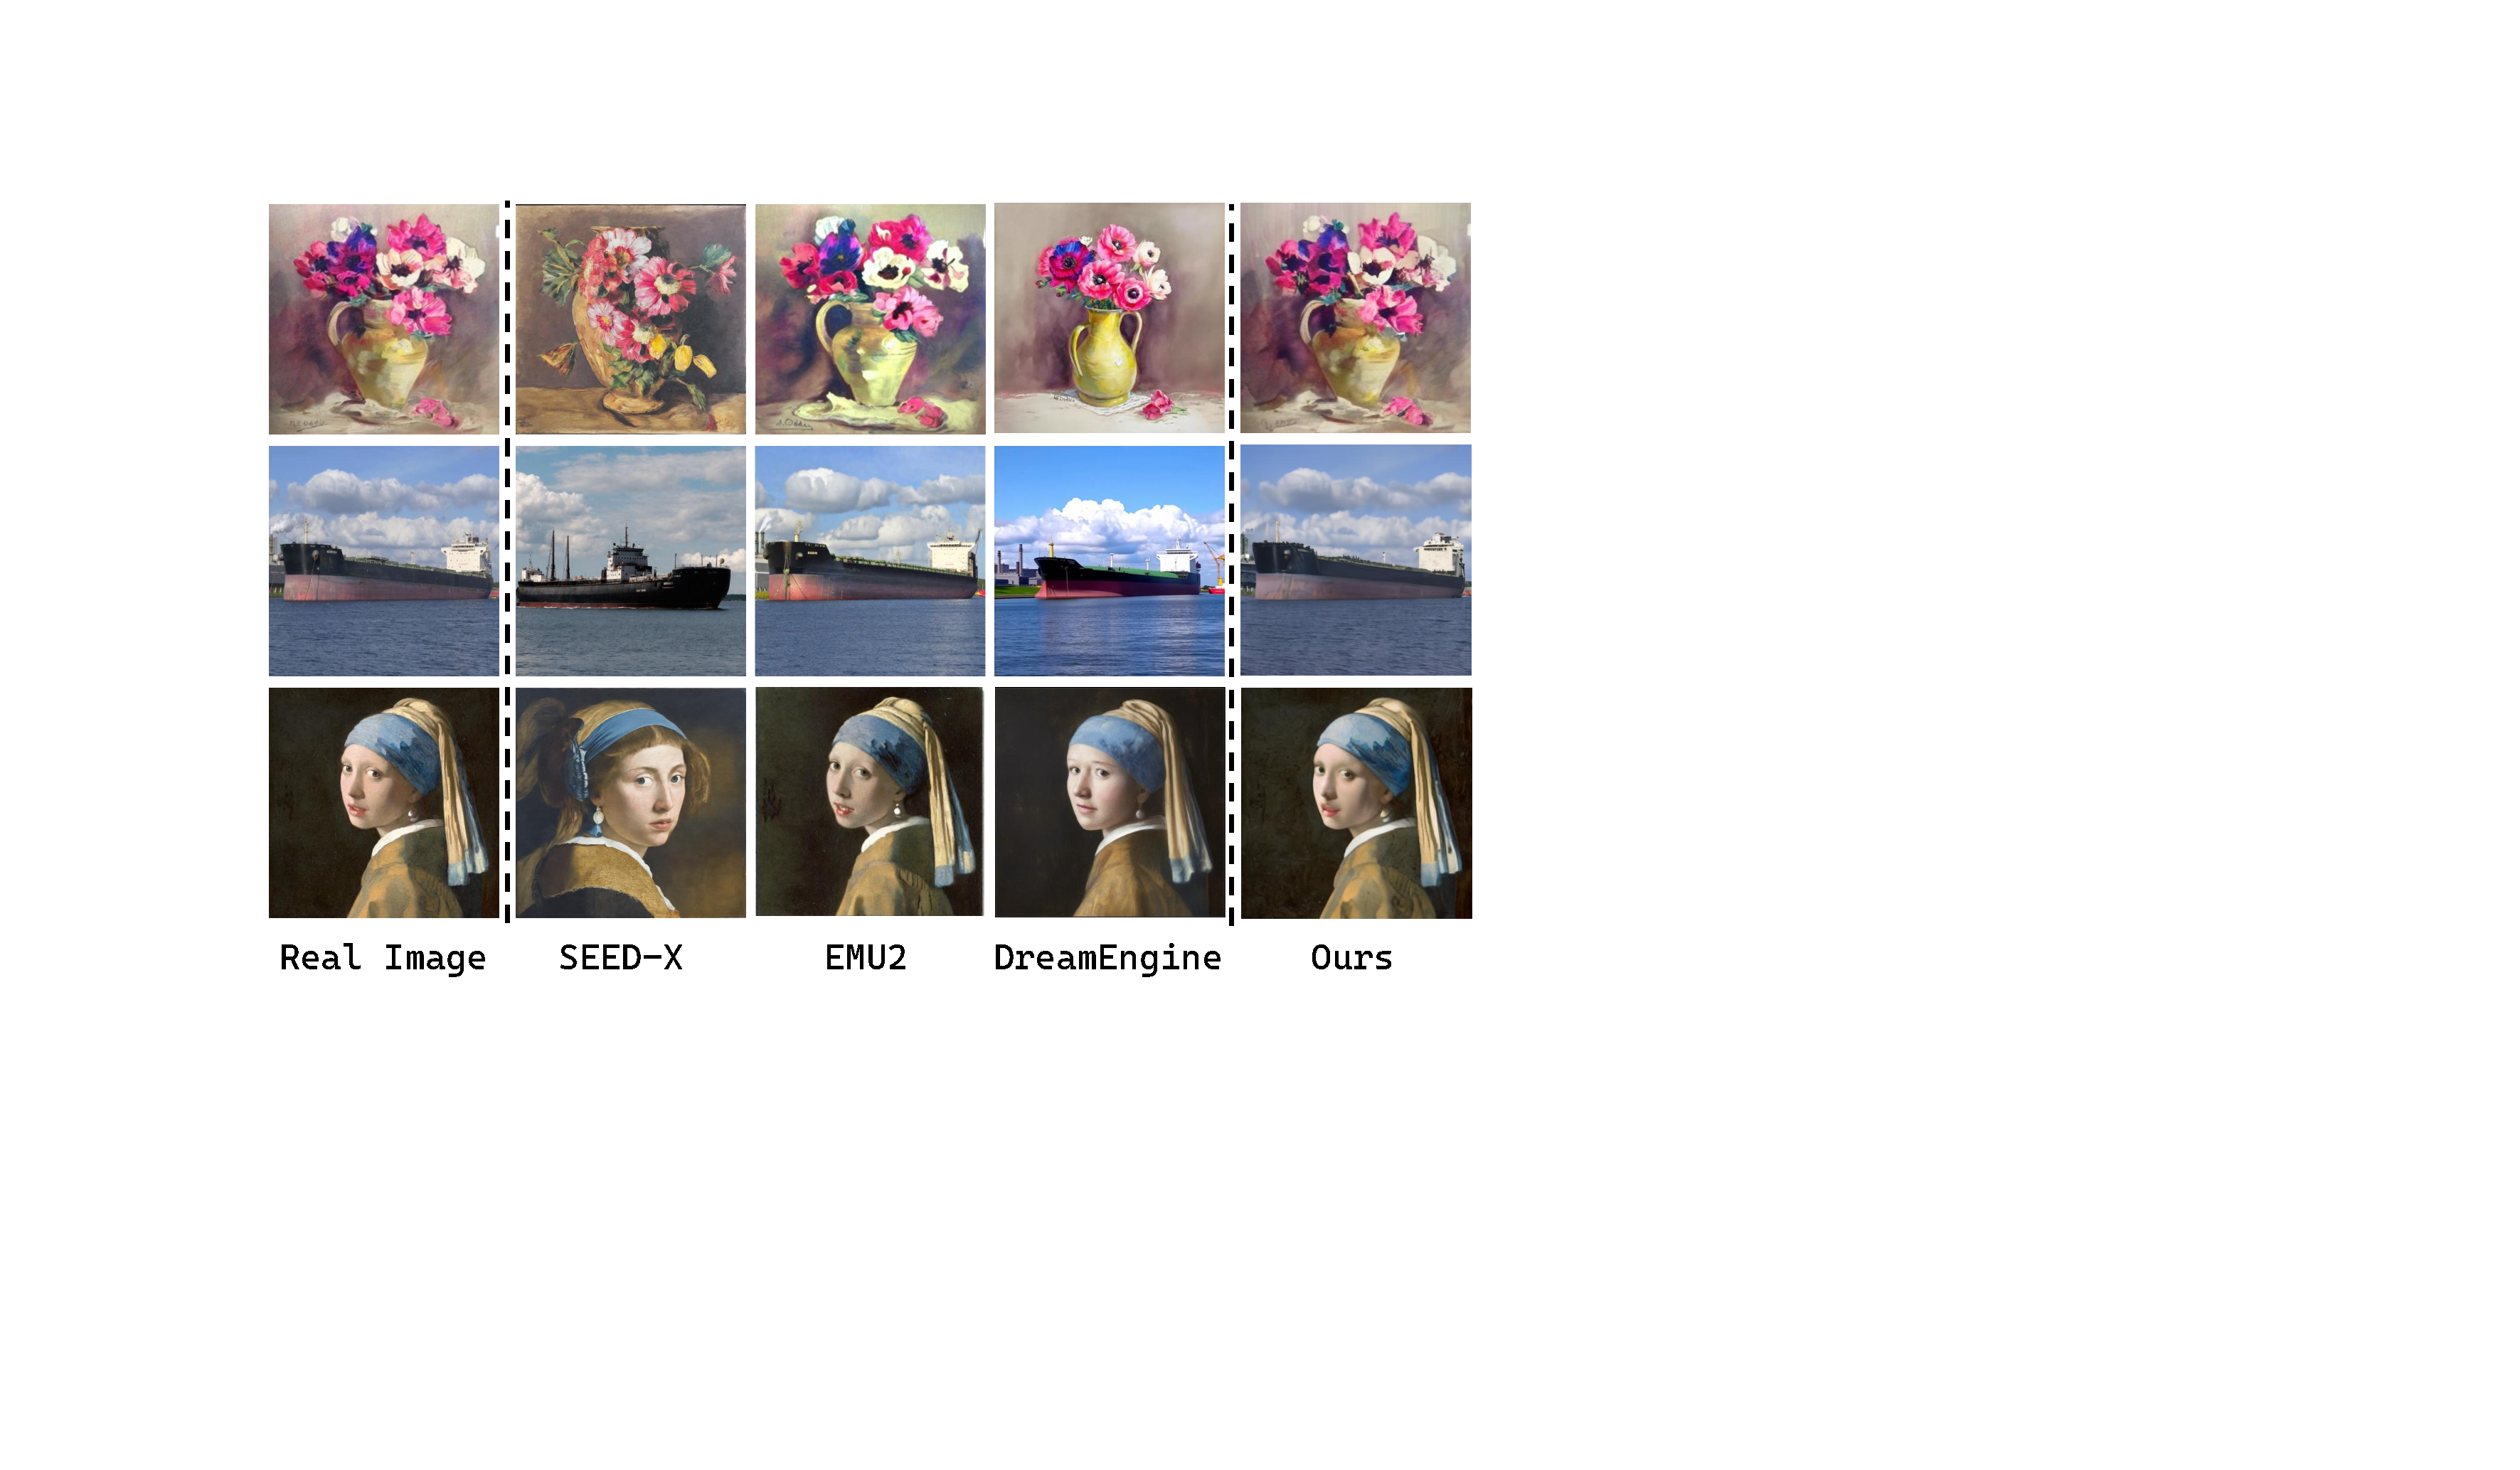
\includegraphics[width=1.0\textwidth]{figures/reconstruction_exp.pdf}
% \caption{Comparison of image reconstruction results among different methods~\citep{dreamengine,2024SeedX,emu2}.}
% \label{fig:reconstruction}
% \end{figure*}


% \begin{table}[t]
% \centering
% \caption{Image reconstruction performance comparison on COCO and JourneyDB datasets.}
% \label{tab:reconstruct}
% \resizebox{0.47\textwidth}{!}{
% \begin{tabular}{@{}lcccc@{}}
% \toprule
% \multirow{2}{*}{\textbf{Method}} & \multicolumn{2}{c}{\textbf{COCO}} & \multicolumn{2}{c}{\textbf{JourneyDB}} \\
% \cmidrule(lr){2-3} \cmidrule(lr){4-5}
%  & CLIP~($\uparrow$) & L2~($\downarrow$) & CLIP~($\uparrow$) & L2~($\downarrow$) \\
% \midrule
% SeedTokenizer              & 0.7760          & 0.5102          & 0.7921          & 0.5291 \\
% EMU2-Gen                  & 0.8537          & \underline{0.3828} & \textbf{0.9299} & \underline{0.2869} \\
% SEED-X                    & \underline{0.8595} & 0.4317          & 0.9017          & 0.4352 \\
% DreamEngine               & \textbf{0.8714} & 0.2065          & 0.9221          & 0.2052 \\

% \midrule
% Ours & 0.8335          & \textbf{0.1008}    & \underline{0.9062}   & \textbf{0.0867} \\
% \bottomrule
% \end{tabular}
% }
% \end{table}







% \paragraph{Image Segmentation}


% BLIP

% Llava

% Diffusion (Kosmos-G with our 1 stage training)


% \paragraph{Generation with Text-Image Interleaved Control}

% Upon completing Stage 2 training, our model gains the ability to integrate multimodal control within the image generation process. To assess our proposed paradigm of image generation capability under text-image interleaved control, we further train the model using a mixture of multi-image data. 

% In this paper, we demonstrate several applications of the model and evaluate its performance against Emu-2~\citep{emu2}, the most pertinent baseline which also facilitates text-image interleaved control.


